\documentclass[addpoints]{exam}
\usepackage{preamble}
\sisetup{group-separator = {,}}
% \setlength\parskip{5pt}

\pagestyle{headandfoot}
\runningheadrule

\firstpagefooter{Access for free at \href{\openstax}{\openstax}}{}{}
\runningfooter{Access for free at \href{\openstax}{\openstax}}{}{}


\firstpageheader{Astronomy}{Test}{Chapter 5: {\small Radiation and Spectra}}


\CorrectChoiceEmphasis{\color{red}\bfseries}
\SolutionEmphasis{\color{red}}
\printanswers

\begin{document}
\begin{questions}


\question
Wavelength is \fillin\ .

\begin{choices}
    \choice the vertical distance between neighboring crests in a wave
    \choice the distance between a crest and a trough in a wave
    \choice the distance traveled by a wave in 1 second 
    \correctchoice the horizontal distance between neighboring crests in a wave
\end{choices}

\question
What is a wave cycle?

\begin{choices}
    \correctchoice the portion of a wave encompassed by 1 wavelength
    \choice the distance from a crest to a trough
    \choice a series of waves in the ocean
    \choice the time it takes a wave to vibrate
\end{choices}

\question
How many wave cycles are shown below?

\begin{figure}[h!]
    \centering
    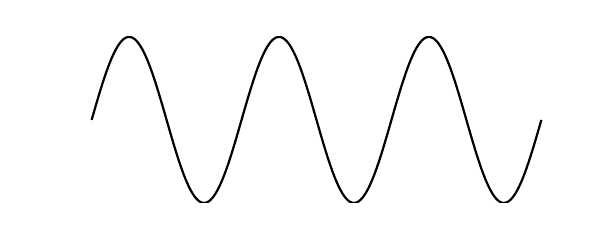
\begin{tikzpicture}
    \def\waveStart{0} %pi/2, pi, 3*pi/2, 0
    \def\nWaves{3}
    \begin{axis}[width=240pt,height=105pt,
        yticklabels={,,},
        xticklabels={,,},
        axis line style={draw=none},
        tick style={draw=none},   
        ymin=-1,
        ymax=1,
    ]
    \addplot[thick, color=black,
        domain=\waveStart:\waveStart+2*pi*\nWaves,
        samples=250]
        {sin(deg((x))};
    \end{axis}
    \end{tikzpicture}
\end{figure}

\begin{oneparchoices}
    \choice 3.5
    \correctchoice 3
    \choice 7
    \choice 6
\end{oneparchoices}

\question
How many wave cycles are shown below?
\begin{figure}[h!]
    \centering
    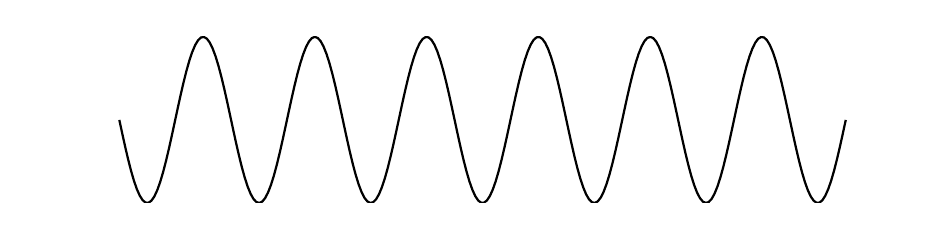
\begin{tikzpicture}
    \def\waveStart{pi} %pi/2, pi, 3*pi/2, 0
    \def\nWaves{6.5}
    \begin{axis}[width=360pt,height=105pt,
        yticklabels={,,},
        xticklabels={,,},
        axis line style={draw=none},
        tick style={draw=none},   
        ymin=-1,
        ymax=1,
    ]
    \addplot[thick, color=black,
        domain=\waveStart:\waveStart+2*pi*\nWaves,
        samples=250]
        {sin(deg((x))};
    \end{axis}
    \end{tikzpicture}
\end{figure}

\begin{oneparchoices}
    \choice 6
    \choice 12
    \correctchoice 6.5
    \choice 13
\end{oneparchoices}

\question
What is electromagnetic radiation?

\begin{choices}
    \choice the portion of a wave encompassed by 1 wave cycle
    \choice toxic gases that travel in waves through the air
    \choice electrons moving through a magnetic field
    \correctchoice waves of combined electric and magnetic fields moving at light-speed
\end{choices}

\question
What is a photon?

\begin{choices}
    \choice a small portion of an electromagnetic wave
    \choice a subatomic particle in the nucleus 
    \correctchoice a particle of light; a unit of electromagnetic radiation
    \choice the uppermost part of a wave
\end{choices}

\question
What are the seven regions of the electromagnetic spectrum?

\begin{choices}
    \choice red, orange, yellow, green, blue, indigo, violet
    \correctchoice radio, microwave, infrared, visible light, ultraviolet, X-ray, gamma ray
    \choice radio, microwave, infrared, green, blue, indigo, violet
    \choice red, orange, yellow, green, ultraviolet, X-ray, gamma ray
\end{choices}

\question
Which type of electromagnetic wave has the \textit{highest} energy?

\begin{choices}
    \choice visible light
    \choice radio
    \choice X-ray
    \correctchoice gamma ray
\end{choices}

\question
Which type of electromagnetic wave has the \textit{lowest} energy?

\begin{choices}
    \choice ultraviolet
    \correctchoice radio
    \choice microwaves
    \choice infrared
\end{choices}

\question
What is the range of wavelength, in nanometers (nm), for visible light?

\begin{choices}
    \choice 0.01--\SI{20}{nm}
    \choice $10^6$--$10^9\,$nm
    \correctchoice 400--\SI{700}{nm}
    \choice 20--\SI{400}{nm}
\end{choices}

% \question
% The frequency of an electromagnetic wave is given by the equation below:

% \begin{equation*}
%     f = \frac{c}{\lambda}\ ,
% \end{equation*}

% where $c = \SI{3e8}{m/s}$ is the speed of light and $\lambda$ is wavelength in meters. What is the frequency of a green light wave with a wavelength of \SI{525}{nm}? (Note: \SI{1}{nm} = \SI{1e-9}{m}.) 
% \textit{Tip}: Use \href{https://www.desmos.com/scientific}{desmos.com/scientific}

\question
What do we see when telescopic instruments capture the Sun in wavelengths outside of the visible light portion of the spectrum, like in X-ray, ultraviolet, or infrared?

\begin{choices}
    \choice Nothing; the Sun is not visible outside the visible portion of the spectrum
    \choice the Sun's rings become apparent
    \choice The true color of the Sun is green
    \correctchoice New parts of the Sun that are normally not visible in normal photographs
\end{choices}

\question
What did Newton discover about sunlight using the apparatus below?

\begin{figure}[h!]
    \centering
    \includegraphics[width=2in]{Figures/Figure5.9.jpg}
\end{figure}

\begin{choices}
    \correctchoice sunlight is made of the colors of the the rainbow
    \choice sunlight contains infrared light
    \choice some colors are warmer than others
    \choice the spectrum contains dark vertical lines
\end{choices}

\question
The figure below is the spectrum of the Sun. What causes the dark lines?

\begin{figure}[h!]
    \centering
    \includegraphics[width=2.5in]{Figures/Figure5.11.jpg}
\end{figure}

\begin{choices}
    \choice imperfections in the manufacturing of the prism
    \choice Earth's atmosphere 
    \choice infrared light waves
    \correctchoice atoms in the Sun absorbing particular wavelengths of light
\end{choices}

\question
Jules Janssen was the first to observe the presence of helium in the Sun. The yellow spectral line for helium was very close to the sodium doublet lines. What is the approximate wavelength of these lines, in nanometers?

\begin{choices}
    \choice \SI{100}{nm}
    \choice \SI{325}{nm}
    \correctchoice \SI{589}{nm}
    \choice \SI{700}{nm}
\end{choices}

\question
How do we know what the Sun is made of?

\begin{choices}
    \choice We collect samples and bring them back to Earth.
    \choice We capture its light and see what the light is made of.
    \choice We actually don't know what the Sun is made of.
    \correctchoice We analyze the absorption lines in its spectrum.
\end{choices}


\end{questions}
\end{document}